%%
%% If you intend to use figures of formats jpg, png or pdf and want the
%% output to be immediately a pdf file, compile with pdflatex.
%%
%% If you want to use eps or ps figures, your output will be a dvi
%% file that can be converted to ps and pdf formats. In this case you
%% should compile your document with latex.
%%
%%This template is compatible with both methods.
%%
\title{{\normalsize Optimization and Algorithms} \\
Financial portfolio optimization}
\author{
        Bernardo Gomes
        \and
        Kishan Rama
        \and
        Tom\'as Falcato \\ {\tt bernardo.n.gomes@ist.utl.pt} \and {\tt kishan.rama@ist.utl.pt} \and {\tt tomas.falcato.costa@ist.utl.pt} \\
        Instituto Superior T\'{e}cnico}
\date{\today}


\documentclass[a4paper]{IEEEtran}
\usepackage[portuguese]{babel}
\usepackage[utf8]{inputenc}
\usepackage{graphicx}
\usepackage{amsmath}
\usepackage{amsfonts}

\begin{document}
\maketitle

\begin{abstract}
  The abstract is the show case of your work. Typically it extends for
  not more than 100-150 words.
  The abstract must not contain references, as it may be used without
  the main article. Avoid general motivation and highlight not just
  the problem, but also the principal results. Usually people read
  abstracts and then decide whether to continue reading the rest of the
  paper. Since the abstract might be used by search engines, be sure
  that terms that identify your work are found there.

\end{abstract}

\section{Introduction}
\label{sec:introduction}
Explain clearly the problem that you address. Use words only, i.e., 
avoid math (this will be given later).

Motivate the problem. At a high level, what is the problem
area you are working in and why is it important? Then, zoom in to the
specific problem considered in this paper.

Finally, summarize what are the main contributions of your paper given
the context you have established in the previous paragraphs. What is
the general approach taken? Why are the specific results significant?


For the paper outline you can write something like: ``The remainder of
the paper is organized as follows. In
Section~\ref{sec:problem-formulation}, we
introduce... Section~\ref{sec:approach} describes ... Numerical
results of... are presented in
Section~\ref{sec:numerical-results}. Finally, we state our conclusions
in Section~\ref{sec:conclusion}.'' Note that Section is capitalized.

\section{Problem formulation}
\label{sec:problem-formulation}

You now introduce the optimization problem to be solved. Explain the
variables used. Mention which ones are optimization variables. Write
the problem formulation \textit{e.g.}, as
\begin{equation}
  \label{eq:problem}
\begin{array}[t]{ll} \text{minimize} & x^\top A x + b^\top x \\
\text{subject to} & C x \leq d \\ & \left\| x - p \right\| \leq 1 \end{array}
\end{equation}
noticing that the equations are part of the text flow, so they are also
punctuated, when needed.

\section{Approach}
\label{sec:approach}

Here you describe what you have done to solve the problem stated in
equation~\eqref{eq:problem}. Whenever you use a result or an algorithm
from a book or a paper, or when you want to refer to some other work,
don't forget to cite it. In \cite{Oetiker11}, you can find further
information about bibliography.

In this document I have included one reference: the number in brackets
in the previous paragraph. At the end of the document you can see the
full reference.

\section{Numerical results}
\label{sec:numerical-results}

How does it really work in practice? Provide simulated performance
metrics. If possible, compare with other well-known methods.

Explain your experiments' setup to make it easily understandable and
replicable by a reader from the field that does not know your problem.

Comment your results. It might help to show a plot, as to illustrate
your commentary, like Figure~\ref{fig:solution-l1}.


The commentary of the plots should not just repeat the graphically
obvious such as "the solution is different from the original signal",
but explain, for example, how this difference relates to quick changes
on the signal. Is the solution too slow to follow the signal
variations? What is the magnitude of the error?

\begin{figure}[htp]
  \centering
  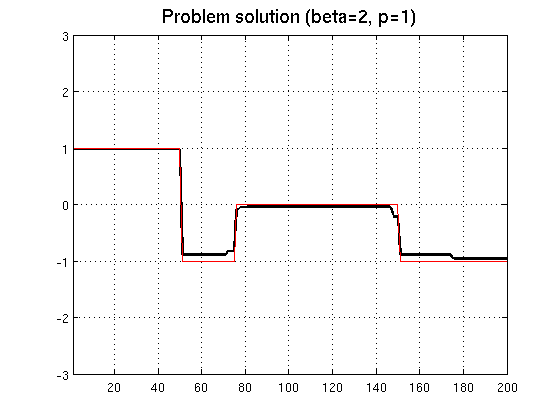
\includegraphics[width=0.9\columnwidth]{./solution1}
  \caption{Solution for the L1 norm cost function.}
  \label{fig:solution-l1}
\end{figure}

You might also want to vary the problem's parameters and see how the
solution evolves. Don't forget to explain why is the choice of
parameters in the solution depicted in Figure~\ref{fig:solution-l1}
better than the others.

Figures should be chosen wisely. You can never lay out the whole
parameter space, so provide insight into which parameters are
significant over what range and which ones are less important.



\section{Conclusions}
\label{sec:conclusion}

In general a short summarizing paragraph will be sufficient. It should
not simply repeat material from the Abstract or Introduction. In some
cases it's possible to now make the original claims more concrete,
\textit{e.g.}, by referring to quantitative results.


\begin{thebibliography}{9}

\bibitem{Oetiker11}
  Tobias Oetiker,
  \emph{The (not so) short introduction to \LaTeX}.
  available at \texttt{http://tobi.oetiker.ch/lshort/lshort.pdf}
  2011

\end{thebibliography}

\end{document}
This is never printed 